% Created 2014-01-02 Thu 16:27
\documentclass[english,presentation]{pivotalbeamer}
                              \subtitle{Example Presentation}
\usetheme{default}
\author{Ronert Obst, Data Scientist}
\date{\today}
\title{Pivotal Beamer Template}
\hypersetup{
  pdfkeywords={},
  pdfsubject={},
  pdfcreator={Emacs 24.3.1 (Org mode 8.2.4)}}
\begin{document}

\maketitle
\begin{frame}{Outline}
\tableofcontents
\end{frame}

\section{First Section}
\label{sec-1}
\begin{frame}[fragile,label=sec-1-1]{Buzzwords}
\begin{itemize}
\item Big data
\begin{enumerate}
\item Next generation data science
\item Elastic deep learning
\end{enumerate}
\item Industry 8.0
\item IoT 5.0
\item More cloud $\rightarrow$ more winning
\end{itemize}
\end{frame}

\begin{frame}[fragile,label=sec-1-2]{Two columns}
\begin{columns}
\begin{column}{0.5\textwidth}
\begin{itemize}
\item Considering the aspect ratio is 16:9
\item It is probably a good idea to use two columns
\item To avoid really long lines
\item Typesetting just looks nicer than in \textbf{PowerPoint}
\item And it can be versioned!
\end{itemize}
\end{column}

\begin{column}{0.5\textwidth}
\begin{itemize}
\item Some other content on this side
\item Big data
\item More big data
\item Hadoop
\item GPDB
\item MADlib
\item $x+\mathbf{y} = z$
\end{itemize}
\end{column}
\end{columns}
\end{frame}

\begin{frame}[fragile,label=sec-1-3]{Let us create a plot with \texttt{ggplot2}}
 \begin{itemize}
\item \texttt{ggplot2} is a really nice plotting library
\item It can export graphics using TikZ
\item Which look really nice in \LaTeX
\end{itemize}

\begin{minted}[bgcolor=bg,fontsize=\scriptsize,linenos=true]{r}
library(ggplot2)
library(gcookbook)
sps <- ggplot(heightweight, aes(x=ageYear, y=heightIn, colour=sex))
+ geom_point()
+ scale_colour_brewer(palette="Set1")
sps + geom_smooth()
\end{minted}
\end{frame}

\begin{frame}[fragile,label=sec-1-4]{The plot using TikZ}
\begin{centering}
\scriptsize{% Created by tikzDevice version 0.6.2 on 2013-02-23 10:26:20
% !TEX encoding = UTF-8 Unicode
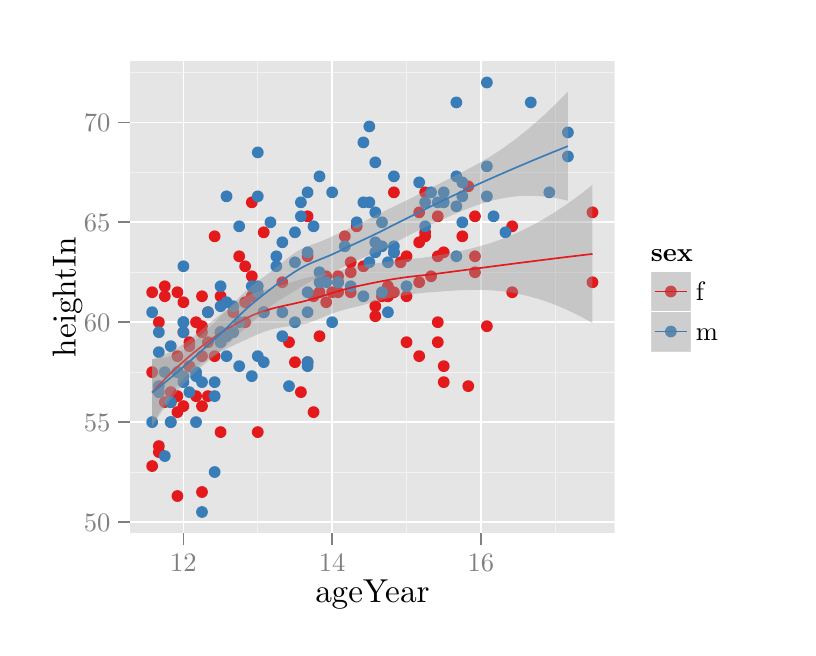
\begin{tikzpicture}[x=1pt,y=1pt]
\definecolor[named]{drawColor}{rgb}{0.00,0.00,0.00}
\definecolor[named]{fillColor}{rgb}{1.00,1.00,1.00}
\fill[color=fillColor,fill opacity=0.00,] (0,0) rectangle (274.63,216.81);
\begin{scope}
\path[clip] (  0.00,  0.00) rectangle (274.63,216.81);
\end{scope}
\begin{scope}
\path[clip] (  0.00,  0.00) rectangle (274.63,216.81);
\end{scope}
\begin{scope}
\path[clip] (  0.00,  0.00) rectangle (274.63,216.81);
\definecolor[named]{drawColor}{rgb}{1.00,1.00,1.00}
\definecolor[named]{fillColor}{rgb}{1.00,1.00,1.00}

\draw[color=drawColor,line width= 0.6pt,line cap=round,line join=round,fill=fillColor,] ( -0.00,  0.00) rectangle (274.63,216.81);
\end{scope}
\begin{scope}
\path[clip] (  0.00,  0.00) rectangle (274.63,216.81);
\end{scope}
\begin{scope}
\path[clip] (  0.00,  0.00) rectangle (274.63,216.81);
\end{scope}
\begin{scope}
\path[clip] (  0.00,  0.00) rectangle (274.63,216.81);
\end{scope}
\begin{scope}
\path[clip] ( 37.02, 34.04) rectangle (212.05,204.77);
\definecolor[named]{fillColor}{rgb}{0.90,0.90,0.90}

\draw[fill=fillColor,draw opacity=0.00,] ( 37.02, 34.04) rectangle (212.05,204.77);
\definecolor[named]{drawColor}{rgb}{0.95,0.95,0.95}

\draw[color=drawColor,line width= 0.3pt,line join=round,fill opacity=0.00,] ( 37.02, 56.24) --
	(212.05, 56.24);

\draw[color=drawColor,line width= 0.3pt,line join=round,fill opacity=0.00,] ( 37.02, 92.33) --
	(212.05, 92.33);

\draw[color=drawColor,line width= 0.3pt,line join=round,fill opacity=0.00,] ( 37.02,128.43) --
	(212.05,128.43);

\draw[color=drawColor,line width= 0.3pt,line join=round,fill opacity=0.00,] ( 37.02,164.52) --
	(212.05,164.52);

\draw[color=drawColor,line width= 0.3pt,line join=round,fill opacity=0.00,] ( 37.02,200.61) --
	(212.05,200.61);

\draw[color=drawColor,line width= 0.3pt,line join=round,fill opacity=0.00,] ( 83.15, 34.04) --
	( 83.15,204.77);

\draw[color=drawColor,line width= 0.3pt,line join=round,fill opacity=0.00,] (136.90, 34.04) --
	(136.90,204.77);

\draw[color=drawColor,line width= 0.3pt,line join=round,fill opacity=0.00,] (190.65, 34.04) --
	(190.65,204.77);
\definecolor[named]{drawColor}{rgb}{1.00,1.00,1.00}

\draw[color=drawColor,line width= 0.6pt,line join=round,fill opacity=0.00,] ( 37.02, 38.19) --
	(212.05, 38.19);

\draw[color=drawColor,line width= 0.6pt,line join=round,fill opacity=0.00,] ( 37.02, 74.28) --
	(212.05, 74.28);

\draw[color=drawColor,line width= 0.6pt,line join=round,fill opacity=0.00,] ( 37.02,110.38) --
	(212.05,110.38);

\draw[color=drawColor,line width= 0.6pt,line join=round,fill opacity=0.00,] ( 37.02,146.47) --
	(212.05,146.47);

\draw[color=drawColor,line width= 0.6pt,line join=round,fill opacity=0.00,] ( 37.02,182.57) --
	(212.05,182.57);

\draw[color=drawColor,line width= 0.6pt,line join=round,fill opacity=0.00,] ( 56.27, 34.04) --
	( 56.27,204.77);

\draw[color=drawColor,line width= 0.6pt,line join=round,fill opacity=0.00,] (110.02, 34.04) --
	(110.02,204.77);

\draw[color=drawColor,line width= 0.6pt,line join=round,fill opacity=0.00,] (163.78, 34.04) --
	(163.78,204.77);
\definecolor[named]{fillColor}{rgb}{0.89,0.10,0.11}

\draw[fill=fillColor,draw opacity=0.00,] ( 54.12, 83.67) circle (  2.13);

\draw[fill=fillColor,draw opacity=0.00,] ( 81.00,126.98) circle (  2.13);

\draw[fill=fillColor,draw opacity=0.00,] ( 76.43,134.20) circle (  2.13);

\draw[fill=fillColor,draw opacity=0.00,] ( 94.43,103.16) circle (  2.13);

\draw[fill=fillColor,draw opacity=0.00,] (161.63,128.43) circle (  2.13);

\draw[fill=fillColor,draw opacity=0.00,] (116.74,128.43) circle (  2.13);

\draw[fill=fillColor,draw opacity=0.00,] (148.19,103.16) circle (  2.13);

\draw[fill=fillColor,draw opacity=0.00,] ( 51.70, 85.11) circle (  2.13);

\draw[fill=fillColor,draw opacity=0.00,] ( 92.02,124.82) circle (  2.13);

\draw[fill=fillColor,draw opacity=0.00,] ( 47.40, 65.62) circle (  2.13);

\draw[fill=fillColor,draw opacity=0.00,] ( 44.98,121.21) circle (  2.13);

\draw[fill=fillColor,draw opacity=0.00,] (132.33,121.21) circle (  2.13);

\draw[fill=fillColor,draw opacity=0.00,] ( 85.30,142.86) circle (  2.13);

\draw[fill=fillColor,draw opacity=0.00,] ( 67.56, 98.11) circle (  2.13);

\draw[fill=fillColor,draw opacity=0.00,] ( 54.12, 47.57) circle (  2.13);

\draw[fill=fillColor,draw opacity=0.00,] ( 58.42,101.72) circle (  2.13);

\draw[fill=fillColor,draw opacity=0.00,] (161.63,148.64) circle (  2.13);

\draw[fill=fillColor,draw opacity=0.00,] ( 69.71,106.77) circle (  2.13);

\draw[fill=fillColor,draw opacity=0.00,] ( 62.99,119.76) circle (  2.13);

\draw[fill=fillColor,draw opacity=0.00,] (136.90,134.20) circle (  2.13);

\draw[fill=fillColor,draw opacity=0.00,] ( 49.55,123.37) circle (  2.13);

\draw[fill=fillColor,draw opacity=0.00,] ( 47.40, 63.45) circle (  2.13);

\draw[fill=fillColor,draw opacity=0.00,] (101.15, 95.94) circle (  2.13);

\draw[fill=fillColor,draw opacity=0.00,] (128.03,119.76) circle (  2.13);

\draw[fill=fillColor,draw opacity=0.00,] (148.19,134.20) circle (  2.13);

\draw[fill=fillColor,draw opacity=0.00,] (105.45,121.21) circle (  2.13);

\draw[fill=fillColor,draw opacity=0.00,] (125.61,116.15) circle (  2.13);

\draw[fill=fillColor,draw opacity=0.00,] (136.90,103.16) circle (  2.13);

\draw[fill=fillColor,draw opacity=0.00,] (204.09,150.08) circle (  2.13);

\draw[fill=fillColor,draw opacity=0.00,] ( 60.84, 83.67) circle (  2.13);

\draw[fill=fillColor,draw opacity=0.00,] (114.59,141.42) circle (  2.13);

\draw[fill=fillColor,draw opacity=0.00,] ( 96.58, 95.94) circle (  2.13);

\draw[fill=fillColor,draw opacity=0.00,] ( 67.56,141.42) circle (  2.13);

\draw[fill=fillColor,draw opacity=0.00,] ( 44.98, 92.33) circle (  2.13);

\draw[fill=fillColor,draw opacity=0.00,] (150.34, 94.50) circle (  2.13);

\draw[fill=fillColor,draw opacity=0.00,] (175.07,121.21) circle (  2.13);

\draw[fill=fillColor,draw opacity=0.00,] (112.17,126.98) circle (  2.13);

\draw[fill=fillColor,draw opacity=0.00,] (130.18,123.37) circle (  2.13);

\draw[fill=fillColor,draw opacity=0.00,] (148.19,148.64) circle (  2.13);

\draw[fill=fillColor,draw opacity=0.00,] (141.47, 98.11) circle (  2.13);

\draw[fill=fillColor,draw opacity=0.00,] (121.31,130.59) circle (  2.13);

\draw[fill=fillColor,draw opacity=0.00,] (105.45,105.32) circle (  2.13);

\draw[fill=fillColor,draw opacity=0.00,] (110.02,121.21) circle (  2.13);

\draw[fill=fillColor,draw opacity=0.00,] (112.17,124.82) circle (  2.13);

\draw[fill=fillColor,draw opacity=0.00,] ( 69.71,119.76) circle (  2.13);

\draw[fill=fillColor,draw opacity=0.00,] (145.77,126.98) circle (  2.13);

\draw[fill=fillColor,draw opacity=0.00,] ( 44.98, 58.40) circle (  2.13);

\draw[fill=fillColor,draw opacity=0.00,] ( 62.99,108.93) circle (  2.13);

\draw[fill=fillColor,draw opacity=0.00,] ( 56.27,106.77) circle (  2.13);

\draw[fill=fillColor,draw opacity=0.00,] (130.18,119.76) circle (  2.13);

\draw[fill=fillColor,draw opacity=0.00,] (132.33,135.64) circle (  2.13);

\draw[fill=fillColor,draw opacity=0.00,] (175.07,145.03) circle (  2.13);

\draw[fill=fillColor,draw opacity=0.00,] ( 60.84,110.38) circle (  2.13);

\draw[fill=fillColor,draw opacity=0.00,] ( 58.42,103.16) circle (  2.13);

\draw[fill=fillColor,draw opacity=0.00,] ( 62.99, 80.06) circle (  2.13);

\draw[fill=fillColor,draw opacity=0.00,] ( 58.42, 94.50) circle (  2.13);

\draw[fill=fillColor,draw opacity=0.00,] ( 81.00,119.76) circle (  2.13);

\draw[fill=fillColor,draw opacity=0.00,] (107.87,126.98) circle (  2.13);

\draw[fill=fillColor,draw opacity=0.00,] (143.62,141.42) circle (  2.13);

\draw[fill=fillColor,draw opacity=0.00,] ( 54.12, 77.89) circle (  2.13);

\draw[fill=fillColor,draw opacity=0.00,] (143.62,142.86) circle (  2.13);

\draw[fill=fillColor,draw opacity=0.00,] (148.19,110.38) circle (  2.13);

\draw[fill=fillColor,draw opacity=0.00,] ( 65.14, 83.67) circle (  2.13);

\draw[fill=fillColor,draw opacity=0.00,] ( 62.99, 98.11) circle (  2.13);

\draw[fill=fillColor,draw opacity=0.00,] ( 78.58,110.38) circle (  2.13);

\draw[fill=fillColor,draw opacity=0.00,] ( 83.15, 70.67) circle (  2.13);

\draw[fill=fillColor,draw opacity=0.00,] ( 56.27, 80.06) circle (  2.13);

\draw[fill=fillColor,draw opacity=0.00,] ( 78.58,130.59) circle (  2.13);

\draw[fill=fillColor,draw opacity=0.00,] ( 74.28,113.99) circle (  2.13);

\draw[fill=fillColor,draw opacity=0.00,] (161.63,134.20) circle (  2.13);

\draw[fill=fillColor,draw opacity=0.00,] (159.21,159.47) circle (  2.13);

\draw[fill=fillColor,draw opacity=0.00,] ( 47.40,110.38) circle (  2.13);

\draw[fill=fillColor,draw opacity=0.00,] ( 65.14,113.99) circle (  2.13);

\draw[fill=fillColor,draw opacity=0.00,] (157.06,141.42) circle (  2.13);

\draw[fill=fillColor,draw opacity=0.00,] ( 54.12, 98.11) circle (  2.13);

\draw[fill=fillColor,draw opacity=0.00,] (132.33,157.30) circle (  2.13);

\draw[fill=fillColor,draw opacity=0.00,] (101.15,148.64) circle (  2.13);

\draw[fill=fillColor,draw opacity=0.00,] ( 85.30,113.99) circle (  2.13);

\draw[fill=fillColor,draw opacity=0.00,] ( 62.99,106.77) circle (  2.13);

\draw[fill=fillColor,draw opacity=0.00,] ( 65.14,103.16) circle (  2.13);

\draw[fill=fillColor,draw opacity=0.00,] (130.18,119.76) circle (  2.13);

\draw[fill=fillColor,draw opacity=0.00,] (116.74,121.21) circle (  2.13);

\draw[fill=fillColor,draw opacity=0.00,] (118.89,145.03) circle (  2.13);

\draw[fill=fillColor,draw opacity=0.00,] (159.21, 87.28) circle (  2.13);

\draw[fill=fillColor,draw opacity=0.00,] (143.62,157.30) circle (  2.13);

\draw[fill=fillColor,draw opacity=0.00,] ( 54.12,121.21) circle (  2.13);

\draw[fill=fillColor,draw opacity=0.00,] (134.75,132.03) circle (  2.13);

\draw[fill=fillColor,draw opacity=0.00,] (150.34, 88.72) circle (  2.13);

\draw[fill=fillColor,draw opacity=0.00,] (141.47,150.08) circle (  2.13);

\draw[fill=fillColor,draw opacity=0.00,] (141.47,124.82) circle (  2.13);

\draw[fill=fillColor,draw opacity=0.00,] ( 51.70, 81.50) circle (  2.13);

\draw[fill=fillColor,draw opacity=0.00,] (103.30,119.76) circle (  2.13);

\draw[fill=fillColor,draw opacity=0.00,] (103.30, 77.89) circle (  2.13);

\draw[fill=fillColor,draw opacity=0.00,] ( 78.58,117.60) circle (  2.13);

\draw[fill=fillColor,draw opacity=0.00,] ( 69.71, 70.67) circle (  2.13);

\draw[fill=fillColor,draw opacity=0.00,] ( 81.00,153.69) circle (  2.13);

\draw[fill=fillColor,draw opacity=0.00,] ( 98.73, 85.11) circle (  2.13);

\draw[fill=fillColor,draw opacity=0.00,] ( 49.55, 81.50) circle (  2.13);

\draw[fill=fillColor,draw opacity=0.00,] ( 62.99, 49.02) circle (  2.13);

\draw[fill=fillColor,draw opacity=0.00,] (204.09,124.82) circle (  2.13);

\draw[fill=fillColor,draw opacity=0.00,] (116.74,132.03) circle (  2.13);

\draw[fill=fillColor,draw opacity=0.00,] (107.87,117.60) circle (  2.13);

\draw[fill=fillColor,draw opacity=0.00,] (141.47,139.25) circle (  2.13);

\draw[fill=fillColor,draw opacity=0.00,] ( 56.27,117.60) circle (  2.13);

\draw[fill=fillColor,draw opacity=0.00,] (165.93,108.93) circle (  2.13);

\draw[fill=fillColor,draw opacity=0.00,] ( 49.55,119.76) circle (  2.13);

\draw[fill=fillColor,draw opacity=0.00,] (101.15,134.20) circle (  2.13);

\draw[fill=fillColor,draw opacity=0.00,] (150.34,135.64) circle (  2.13);

\draw[fill=fillColor,draw opacity=0.00,] (112.17,121.21) circle (  2.13);

\draw[fill=fillColor,draw opacity=0.00,] (125.61,112.54) circle (  2.13);

\draw[fill=fillColor,draw opacity=0.00,] (136.90,119.76) circle (  2.13);
\definecolor[named]{fillColor}{rgb}{0.22,0.49,0.72}

\draw[fill=fillColor,draw opacity=0.00,] (103.30,145.03) circle (  2.13);

\draw[fill=fillColor,draw opacity=0.00,] ( 85.30,113.99) circle (  2.13);

\draw[fill=fillColor,draw opacity=0.00,] ( 56.27, 90.89) circle (  2.13);

\draw[fill=fillColor,draw opacity=0.00,] ( 69.71,106.77) circle (  2.13);

\draw[fill=fillColor,draw opacity=0.00,] ( 69.71,116.15) circle (  2.13);

\draw[fill=fillColor,draw opacity=0.00,] ( 44.98,113.99) circle (  2.13);

\draw[fill=fillColor,draw opacity=0.00,] (157.06,160.91) circle (  2.13);

\draw[fill=fillColor,draw opacity=0.00,] (143.62,145.03) circle (  2.13);

\draw[fill=fillColor,draw opacity=0.00,] ( 62.99, 41.80) circle (  2.13);

\draw[fill=fillColor,draw opacity=0.00,] ( 60.84, 92.33) circle (  2.13);

\draw[fill=fillColor,draw opacity=0.00,] ( 92.02,113.99) circle (  2.13);

\draw[fill=fillColor,draw opacity=0.00,] ( 83.15,123.37) circle (  2.13);

\draw[fill=fillColor,draw opacity=0.00,] (121.31,119.76) circle (  2.13);

\draw[fill=fillColor,draw opacity=0.00,] ( 71.86,155.86) circle (  2.13);

\draw[fill=fillColor,draw opacity=0.00,] ( 49.55, 62.01) circle (  2.13);

\draw[fill=fillColor,draw opacity=0.00,] ( 69.71,103.16) circle (  2.13);

\draw[fill=fillColor,draw opacity=0.00,] (101.15, 94.50) circle (  2.13);

\draw[fill=fillColor,draw opacity=0.00,] ( 76.43,110.38) circle (  2.13);

\draw[fill=fillColor,draw opacity=0.00,] (195.22,170.29) circle (  2.13);

\draw[fill=fillColor,draw opacity=0.00,] (128.03,137.81) circle (  2.13);

\draw[fill=fillColor,draw opacity=0.00,] (128.03,146.47) circle (  2.13);

\draw[fill=fillColor,draw opacity=0.00,] ( 47.40,106.77) circle (  2.13);

\draw[fill=fillColor,draw opacity=0.00,] (148.19,153.69) circle (  2.13);

\draw[fill=fillColor,draw opacity=0.00,] (136.90,123.37) circle (  2.13);

\draw[fill=fillColor,draw opacity=0.00,] ( 60.84, 90.89) circle (  2.13);

\draw[fill=fillColor,draw opacity=0.00,] (143.62,153.69) circle (  2.13);

\draw[fill=fillColor,draw opacity=0.00,] ( 47.40, 85.11) circle (  2.13);

\draw[fill=fillColor,draw opacity=0.00,] ( 71.86, 98.11) circle (  2.13);

\draw[fill=fillColor,draw opacity=0.00,] ( 71.86,117.60) circle (  2.13);

\draw[fill=fillColor,draw opacity=0.00,] ( 56.27,130.59) circle (  2.13);

\draw[fill=fillColor,draw opacity=0.00,] ( 92.02,105.32) circle (  2.13);

\draw[fill=fillColor,draw opacity=0.00,] (132.33,163.08) circle (  2.13);

\draw[fill=fillColor,draw opacity=0.00,] (165.93,155.86) circle (  2.13);

\draw[fill=fillColor,draw opacity=0.00,] ( 96.58,142.86) circle (  2.13);

\draw[fill=fillColor,draw opacity=0.00,] (101.15,113.99) circle (  2.13);

\draw[fill=fillColor,draw opacity=0.00,] (150.34,153.69) circle (  2.13);

\draw[fill=fillColor,draw opacity=0.00,] ( 54.12, 92.33) circle (  2.13);

\draw[fill=fillColor,draw opacity=0.00,] (125.61,139.25) circle (  2.13);

\draw[fill=fillColor,draw opacity=0.00,] (125.61,168.13) circle (  2.13);

\draw[fill=fillColor,draw opacity=0.00,] (125.61,135.64) circle (  2.13);

\draw[fill=fillColor,draw opacity=0.00,] (121.31,175.35) circle (  2.13);

\draw[fill=fillColor,draw opacity=0.00,] (114.59,137.81) circle (  2.13);

\draw[fill=fillColor,draw opacity=0.00,] (123.46,153.69) circle (  2.13);

\draw[fill=fillColor,draw opacity=0.00,] (101.15,135.64) circle (  2.13);

\draw[fill=fillColor,draw opacity=0.00,] ( 56.27,106.77) circle (  2.13);

\draw[fill=fillColor,draw opacity=0.00,] ( 83.15,155.86) circle (  2.13);

\draw[fill=fillColor,draw opacity=0.00,] ( 67.56, 88.72) circle (  2.13);

\draw[fill=fillColor,draw opacity=0.00,] ( 56.27,110.38) circle (  2.13);

\draw[fill=fillColor,draw opacity=0.00,] ( 62.99, 88.72) circle (  2.13);

\draw[fill=fillColor,draw opacity=0.00,] (154.91,163.08) circle (  2.13);

\draw[fill=fillColor,draw opacity=0.00,] (112.17,124.82) circle (  2.13);

\draw[fill=fillColor,draw opacity=0.00,] (118.89,146.47) circle (  2.13);

\draw[fill=fillColor,draw opacity=0.00,] ( 69.71,106.77) circle (  2.13);

\draw[fill=fillColor,draw opacity=0.00,] (165.93,166.69) circle (  2.13);

\draw[fill=fillColor,draw opacity=0.00,] ( 85.30, 95.94) circle (  2.13);

\draw[fill=fillColor,draw opacity=0.00,] (110.02,110.38) circle (  2.13);

\draw[fill=fillColor,draw opacity=0.00,] ( 47.40, 99.55) circle (  2.13);

\draw[fill=fillColor,draw opacity=0.00,] ( 83.15, 98.11) circle (  2.13);

\draw[fill=fillColor,draw opacity=0.00,] ( 83.15,121.21) circle (  2.13);

\draw[fill=fillColor,draw opacity=0.00,] ( 87.72,146.47) circle (  2.13);

\draw[fill=fillColor,draw opacity=0.00,] (145.77,157.30) circle (  2.13);

\draw[fill=fillColor,draw opacity=0.00,] ( 83.15,171.74) circle (  2.13);

\draw[fill=fillColor,draw opacity=0.00,] ( 56.27, 88.72) circle (  2.13);

\draw[fill=fillColor,draw opacity=0.00,] (128.03,121.21) circle (  2.13);

\draw[fill=fillColor,draw opacity=0.00,] (110.02,157.30) circle (  2.13);

\draw[fill=fillColor,draw opacity=0.00,] ( 67.56, 56.24) circle (  2.13);

\draw[fill=fillColor,draw opacity=0.00,] ( 51.70, 74.28) circle (  2.13);

\draw[fill=fillColor,draw opacity=0.00,] (154.91,189.79) circle (  2.13);

\draw[fill=fillColor,draw opacity=0.00,] (188.50,157.30) circle (  2.13);

\draw[fill=fillColor,draw opacity=0.00,] ( 51.70,101.72) circle (  2.13);

\draw[fill=fillColor,draw opacity=0.00,] (157.06,155.86) circle (  2.13);

\draw[fill=fillColor,draw opacity=0.00,] (154.91,152.25) circle (  2.13);

\draw[fill=fillColor,draw opacity=0.00,] (181.79,189.79) circle (  2.13);

\draw[fill=fillColor,draw opacity=0.00,] ( 74.28,106.77) circle (  2.13);

\draw[fill=fillColor,draw opacity=0.00,] (123.46,181.12) circle (  2.13);

\draw[fill=fillColor,draw opacity=0.00,] (105.45,128.43) circle (  2.13);

\draw[fill=fillColor,draw opacity=0.00,] ( 58.42, 85.11) circle (  2.13);

\draw[fill=fillColor,draw opacity=0.00,] ( 54.12, 92.33) circle (  2.13);

\draw[fill=fillColor,draw opacity=0.00,] ( 98.73,148.64) circle (  2.13);

\draw[fill=fillColor,draw opacity=0.00,] (105.45,163.08) circle (  2.13);

\draw[fill=fillColor,draw opacity=0.00,] (141.47,160.91) circle (  2.13);

\draw[fill=fillColor,draw opacity=0.00,] (121.31,153.69) circle (  2.13);

\draw[fill=fillColor,draw opacity=0.00,] ( 81.00,123.37) circle (  2.13);

\draw[fill=fillColor,draw opacity=0.00,] ( 96.58,110.38) circle (  2.13);

\draw[fill=fillColor,draw opacity=0.00,] (130.18,132.03) circle (  2.13);

\draw[fill=fillColor,draw opacity=0.00,] (130.18,113.99) circle (  2.13);

\draw[fill=fillColor,draw opacity=0.00,] (125.61,150.08) circle (  2.13);

\draw[fill=fillColor,draw opacity=0.00,] (105.45,124.82) circle (  2.13);

\draw[fill=fillColor,draw opacity=0.00,] ( 69.71,103.16) circle (  2.13);

\draw[fill=fillColor,draw opacity=0.00,] ( 69.71,123.37) circle (  2.13);

\draw[fill=fillColor,draw opacity=0.00,] (154.91,134.20) circle (  2.13);

\draw[fill=fillColor,draw opacity=0.00,] ( 98.73,153.69) circle (  2.13);

\draw[fill=fillColor,draw opacity=0.00,] (116.74,123.37) circle (  2.13);

\draw[fill=fillColor,draw opacity=0.00,] ( 96.58,132.03) circle (  2.13);

\draw[fill=fillColor,draw opacity=0.00,] ( 49.55, 92.33) circle (  2.13);

\draw[fill=fillColor,draw opacity=0.00,] (123.46,132.03) circle (  2.13);

\draw[fill=fillColor,draw opacity=0.00,] ( 51.70, 81.50) circle (  2.13);

\draw[fill=fillColor,draw opacity=0.00,] ( 65.14,113.99) circle (  2.13);

\draw[fill=fillColor,draw opacity=0.00,] ( 47.40, 87.28) circle (  2.13);

\draw[fill=fillColor,draw opacity=0.00,] ( 92.02,139.25) circle (  2.13);

\draw[fill=fillColor,draw opacity=0.00,] ( 56.27,110.38) circle (  2.13);

\draw[fill=fillColor,draw opacity=0.00,] (195.22,178.96) circle (  2.13);

\draw[fill=fillColor,draw opacity=0.00,] ( 89.87,134.20) circle (  2.13);

\draw[fill=fillColor,draw opacity=0.00,] ( 67.56, 83.67) circle (  2.13);

\draw[fill=fillColor,draw opacity=0.00,] (165.93,197.00) circle (  2.13);

\draw[fill=fillColor,draw opacity=0.00,] (168.35,148.64) circle (  2.13);

\draw[fill=fillColor,draw opacity=0.00,] ( 74.28,116.15) circle (  2.13);

\draw[fill=fillColor,draw opacity=0.00,] ( 60.84, 74.28) circle (  2.13);

\draw[fill=fillColor,draw opacity=0.00,] ( 44.98, 74.28) circle (  2.13);

\draw[fill=fillColor,draw opacity=0.00,] (150.34,157.30) circle (  2.13);

\draw[fill=fillColor,draw opacity=0.00,] ( 94.43, 87.28) circle (  2.13);

\draw[fill=fillColor,draw opacity=0.00,] ( 76.43,145.03) circle (  2.13);

\draw[fill=fillColor,draw opacity=0.00,] (172.65,142.86) circle (  2.13);

\draw[fill=fillColor,draw opacity=0.00,] (101.15, 95.94) circle (  2.13);

\draw[fill=fillColor,draw opacity=0.00,] ( 89.87,130.59) circle (  2.13);

\draw[fill=fillColor,draw opacity=0.00,] (132.33,137.81) circle (  2.13);

\draw[fill=fillColor,draw opacity=0.00,] ( 76.43, 94.50) circle (  2.13);

\draw[fill=fillColor,draw opacity=0.00,] ( 81.00, 90.89) circle (  2.13);

\draw[fill=fillColor,draw opacity=0.00,] (132.33,135.64) circle (  2.13);

\draw[fill=fillColor,draw opacity=0.00,] ( 51.70, 74.28) circle (  2.13);

\draw[fill=fillColor,draw opacity=0.00,] (101.15,157.30) circle (  2.13);

\draw[fill=fillColor,draw opacity=0.00,] (157.06,146.47) circle (  2.13);

\draw[fill=fillColor,draw opacity=0.00,] (101.15,121.21) circle (  2.13);

\draw[fill=fillColor,draw opacity=0.00,] (107.87,124.82) circle (  2.13);

\draw[fill=fillColor,draw opacity=0.00,] ( 71.86,105.32) circle (  2.13);
\definecolor[named]{fillColor}{rgb}{0.60,0.60,0.60}

\draw[fill=fillColor,fill opacity=0.40,draw opacity=0.00,] ( 44.98, 96.89) --
	( 46.99, 97.62) --
	( 49.01, 98.45) --
	( 51.02, 99.40) --
	( 53.04,100.48) --
	( 55.05,101.70) --
	( 57.06,103.06) --
	( 59.08,104.56) --
	( 61.09,106.17) --
	( 63.11,107.86) --
	( 65.12,109.56) --
	( 67.14,111.21) --
	( 69.15,112.80) --
	( 71.16,114.31) --
	( 73.18,115.76) --
	( 75.19,117.12) --
	( 77.21,118.42) --
	( 79.22,119.63) --
	( 81.23,120.61) --
	( 83.25,121.36) --
	( 85.26,121.96) --
	( 87.28,122.49) --
	( 89.29,123.01) --
	( 91.30,123.56) --
	( 93.32,124.16) --
	( 95.33,124.80) --
	( 97.35,125.43) --
	( 99.36,126.04) --
	(101.37,126.58) --
	(103.39,127.02) --
	(105.40,127.40) --
	(107.42,127.77) --
	(109.43,128.19) --
	(111.45,128.69) --
	(113.46,129.25) --
	(115.47,129.83) --
	(117.49,130.36) --
	(119.50,130.78) --
	(121.52,131.10) --
	(123.53,131.37) --
	(125.54,131.61) --
	(127.56,131.86) --
	(129.57,132.13) --
	(131.59,132.41) --
	(133.60,132.68) --
	(135.61,132.94) --
	(137.63,133.15) --
	(139.64,133.34) --
	(141.66,133.55) --
	(143.67,133.80) --
	(145.68,134.10) --
	(147.70,134.44) --
	(149.71,134.80) --
	(151.73,135.17) --
	(153.74,135.57) --
	(155.76,135.98) --
	(157.77,136.43) --
	(159.78,136.90) --
	(161.80,137.41) --
	(163.81,137.95) --
	(165.83,138.54) --
	(167.84,139.18) --
	(169.85,139.87) --
	(171.87,140.61) --
	(173.88,141.40) --
	(175.90,142.26) --
	(177.91,143.17) --
	(179.92,144.13) --
	(181.94,145.16) --
	(183.95,146.24) --
	(185.97,147.38) --
	(187.98,148.57) --
	(189.99,149.82) --
	(192.01,151.12) --
	(194.02,152.48) --
	(196.04,153.89) --
	(198.05,155.34) --
	(200.07,156.85) --
	(202.08,158.41) --
	(204.09,160.02) --
	(204.09,110.07) --
	(202.08,111.20) --
	(200.07,112.29) --
	(198.05,113.32) --
	(196.04,114.29) --
	(194.02,115.21) --
	(192.01,116.08) --
	(189.99,116.88) --
	(187.98,117.63) --
	(185.97,118.32) --
	(183.95,118.96) --
	(181.94,119.53) --
	(179.92,120.04) --
	(177.91,120.49) --
	(175.90,120.89) --
	(173.88,121.22) --
	(171.87,121.49) --
	(169.85,121.71) --
	(167.84,121.87) --
	(165.83,121.99) --
	(163.81,122.05) --
	(161.80,122.07) --
	(159.78,122.04) --
	(157.77,121.99) --
	(155.76,121.90) --
	(153.74,121.79) --
	(151.73,121.66) --
	(149.71,121.50) --
	(147.70,121.34) --
	(145.68,121.19) --
	(143.67,121.05) --
	(141.66,120.86) --
	(139.64,120.63) --
	(137.63,120.34) --
	(135.61,120.02) --
	(133.60,119.68) --
	(131.59,119.31) --
	(129.57,118.88) --
	(127.56,118.39) --
	(125.54,117.85) --
	(123.53,117.27) --
	(121.52,116.69) --
	(119.50,116.15) --
	(117.49,115.67) --
	(115.47,115.18) --
	(113.46,114.65) --
	(111.45,114.02) --
	(109.43,113.29) --
	(107.42,112.46) --
	(105.40,111.60) --
	(103.39,110.78) --
	(101.37,110.09) --
	( 99.36,109.59) --
	( 97.35,109.26) --
	( 95.33,109.01) --
	( 93.32,108.78) --
	( 91.30,108.48) --
	( 89.29,108.07) --
	( 87.28,107.52) --
	( 85.26,106.83) --
	( 83.25,106.03) --
	( 81.23,105.15) --
	( 79.22,104.23) --
	( 77.21,103.30) --
	( 75.19,102.37) --
	( 73.18,101.42) --
	( 71.16,100.44) --
	( 69.15, 99.41) --
	( 67.14, 98.31) --
	( 65.12, 97.12) --
	( 63.11, 95.81) --
	( 61.09, 94.33) --
	( 59.08, 92.64) --
	( 57.06, 90.70) --
	( 55.05, 88.48) --
	( 53.04, 85.97) --
	( 51.02, 83.16) --
	( 49.01, 80.06) --
	( 46.99, 76.71) --
	( 44.98, 73.14) --
	cycle;
\definecolor[named]{drawColor}{rgb}{0.89,0.10,0.11}
\definecolor[named]{fillColor}{rgb}{0.89,0.10,0.11}

\draw[color=drawColor,line width= 0.6pt,line join=round,] ( 44.98, 85.01) --
	( 46.99, 87.17) --
	( 49.01, 89.26) --
	( 51.02, 91.28) --
	( 53.04, 93.23) --
	( 55.05, 95.09) --
	( 57.06, 96.88) --
	( 59.08, 98.60) --
	( 61.09,100.25) --
	( 63.11,101.83) --
	( 65.12,103.34) --
	( 67.14,104.76) --
	( 69.15,106.10) --
	( 71.16,107.38) --
	( 73.18,108.59) --
	( 75.19,109.75) --
	( 77.21,110.86) --
	( 79.22,111.93) --
	( 81.23,112.88) --
	( 83.25,113.69) --
	( 85.26,114.40) --
	( 87.28,115.00) --
	( 89.29,115.54) --
	( 91.30,116.02) --
	( 93.32,116.47) --
	( 95.33,116.90) --
	( 97.35,117.35) --
	( 99.36,117.82) --
	(101.37,118.34) --
	(103.39,118.90) --
	(105.40,119.50) --
	(107.42,120.12) --
	(109.43,120.74) --
	(111.45,121.36) --
	(113.46,121.95) --
	(115.47,122.51) --
	(117.49,123.02) --
	(119.50,123.47) --
	(121.52,123.90) --
	(123.53,124.32) --
	(125.54,124.73) --
	(127.56,125.13) --
	(129.57,125.50) --
	(131.59,125.86) --
	(133.60,126.18) --
	(135.61,126.48) --
	(137.63,126.75) --
	(139.64,126.98) --
	(141.66,127.21) --
	(143.67,127.42) --
	(145.68,127.65) --
	(147.70,127.89) --
	(149.71,128.15) --
	(151.73,128.41) --
	(153.74,128.68) --
	(155.76,128.94) --
	(157.77,129.21) --
	(159.78,129.47) --
	(161.80,129.74) --
	(163.81,130.00) --
	(165.83,130.26) --
	(167.84,130.53) --
	(169.85,130.79) --
	(171.87,131.05) --
	(173.88,131.31) --
	(175.90,131.57) --
	(177.91,131.83) --
	(179.92,132.09) --
	(181.94,132.34) --
	(183.95,132.60) --
	(185.97,132.85) --
	(187.98,133.10) --
	(189.99,133.35) --
	(192.01,133.60) --
	(194.02,133.85) --
	(196.04,134.09) --
	(198.05,134.33) --
	(200.07,134.57) --
	(202.08,134.81) --
	(204.09,135.04);
\definecolor[named]{fillColor}{rgb}{0.60,0.60,0.60}

\draw[fill=fillColor,fill opacity=0.40,draw opacity=0.00,] ( 44.98, 97.06) --
	( 46.88, 97.15) --
	( 48.78, 97.40) --
	( 50.69, 97.84) --
	( 52.59, 98.50) --
	( 54.49, 99.40) --
	( 56.39,100.55) --
	( 58.29,101.90) --
	( 60.19,103.43) --
	( 62.10,105.10) --
	( 64.00,106.86) --
	( 65.90,108.68) --
	( 67.80,110.50) --
	( 69.70,112.38) --
	( 71.61,114.32) --
	( 73.51,116.30) --
	( 75.41,118.27) --
	( 77.31,120.19) --
	( 79.21,122.00) --
	( 81.11,123.64) --
	( 83.02,125.10) --
	( 84.92,126.47) --
	( 86.82,127.84) --
	( 88.72,129.28) --
	( 90.62,130.82) --
	( 92.53,132.40) --
	( 94.43,133.95) --
	( 96.33,135.35) --
	( 98.23,136.50) --
	(100.13,137.39) --
	(102.03,138.14) --
	(103.94,138.83) --
	(105.84,139.55) --
	(107.74,140.33) --
	(109.64,141.18) --
	(111.54,142.09) --
	(113.45,143.01) --
	(115.35,143.86) --
	(117.25,144.71) --
	(119.15,145.58) --
	(121.05,146.50) --
	(122.95,147.47) --
	(124.86,148.46) --
	(126.76,149.45) --
	(128.66,150.40) --
	(130.56,151.33) --
	(132.46,152.25) --
	(134.37,153.17) --
	(136.27,154.09) --
	(138.17,155.02) --
	(140.07,155.96) --
	(141.97,156.92) --
	(143.87,157.89) --
	(145.78,158.87) --
	(147.68,159.86) --
	(149.58,160.84) --
	(151.48,161.82) --
	(153.38,162.79) --
	(155.29,163.74) --
	(157.19,164.71) --
	(159.09,165.69) --
	(160.99,166.71) --
	(162.89,167.76) --
	(164.79,168.85) --
	(166.70,169.98) --
	(168.60,171.17) --
	(170.50,172.41) --
	(172.40,173.71) --
	(174.30,175.07) --
	(176.21,176.48) --
	(178.11,177.96) --
	(180.01,179.49) --
	(181.91,181.08) --
	(183.81,182.73) --
	(185.71,184.43) --
	(187.62,186.19) --
	(189.52,188.00) --
	(191.42,189.86) --
	(193.32,191.77) --
	(195.22,193.73) --
	(195.22,154.27) --
	(193.32,154.71) --
	(191.42,155.10) --
	(189.52,155.42) --
	(187.62,155.67) --
	(185.71,155.86) --
	(183.81,155.99) --
	(181.91,156.05) --
	(180.01,156.04) --
	(178.11,155.96) --
	(176.21,155.81) --
	(174.30,155.60) --
	(172.40,155.30) --
	(170.50,154.94) --
	(168.60,154.51) --
	(166.70,154.02) --
	(164.79,153.46) --
	(162.89,152.84) --
	(160.99,152.17) --
	(159.09,151.45) --
	(157.19,150.70) --
	(155.29,149.90) --
	(153.38,149.09) --
	(151.48,148.26) --
	(149.58,147.42) --
	(147.68,146.56) --
	(145.78,145.69) --
	(143.87,144.80) --
	(141.97,143.89) --
	(140.07,142.95) --
	(138.17,141.99) --
	(136.27,141.00) --
	(134.37,140.01) --
	(132.46,139.01) --
	(130.56,138.00) --
	(128.66,137.02) --
	(126.76,136.07) --
	(124.86,135.22) --
	(122.95,134.41) --
	(121.05,133.61) --
	(119.15,132.77) --
	(117.25,131.88) --
	(115.35,130.94) --
	(113.45,129.98) --
	(111.54,129.04) --
	(109.64,128.23) --
	(107.74,127.50) --
	(105.84,126.76) --
	(103.94,125.94) --
	(102.03,125.00) --
	(100.13,123.94) --
	( 98.23,122.80) --
	( 96.33,121.59) --
	( 94.43,120.44) --
	( 92.53,119.32) --
	( 90.62,118.14) --
	( 88.72,116.83) --
	( 86.82,115.34) --
	( 84.92,113.72) --
	( 83.02,112.03) --
	( 81.11,110.39) --
	( 79.21,108.77) --
	( 77.31,107.06) --
	( 75.41,105.29) --
	( 73.51,103.50) --
	( 71.61,101.73) --
	( 69.70,100.02) --
	( 67.80, 98.43) --
	( 65.90, 96.92) --
	( 64.00, 95.36) --
	( 62.10, 93.73) --
	( 60.19, 92.00) --
	( 58.29, 90.15) --
	( 56.39, 88.14) --
	( 54.49, 85.97) --
	( 52.59, 83.65) --
	( 50.69, 81.17) --
	( 48.78, 78.53) --
	( 46.88, 75.74) --
	( 44.98, 72.79) --
	cycle;
\definecolor[named]{drawColor}{rgb}{0.22,0.49,0.72}
\definecolor[named]{fillColor}{rgb}{0.22,0.49,0.72}

\draw[color=drawColor,line width= 0.6pt,line join=round,] ( 44.98, 84.92) --
	( 46.88, 86.45) --
	( 48.78, 87.97) --
	( 50.69, 89.50) --
	( 52.59, 91.07) --
	( 54.49, 92.69) --
	( 56.39, 94.34) --
	( 58.29, 96.02) --
	( 60.19, 97.72) --
	( 62.10, 99.42) --
	( 64.00,101.11) --
	( 65.90,102.80) --
	( 67.80,104.46) --
	( 69.70,106.20) --
	( 71.61,108.03) --
	( 73.51,109.90) --
	( 75.41,111.78) --
	( 77.31,113.62) --
	( 79.21,115.38) --
	( 81.11,117.02) --
	( 83.02,118.57) --
	( 84.92,120.10) --
	( 86.82,121.59) --
	( 88.72,123.05) --
	( 90.62,124.48) --
	( 92.53,125.86) --
	( 94.43,127.19) --
	( 96.33,128.47) --
	( 98.23,129.65) --
	(100.13,130.67) --
	(102.03,131.57) --
	(103.94,132.38) --
	(105.84,133.15) --
	(107.74,133.91) --
	(109.64,134.71) --
	(111.54,135.56) --
	(113.45,136.49) --
	(115.35,137.40) --
	(117.25,138.29) --
	(119.15,139.17) --
	(121.05,140.05) --
	(122.95,140.94) --
	(124.86,141.84) --
	(126.76,142.76) --
	(128.66,143.71) --
	(130.56,144.67) --
	(132.46,145.63) --
	(134.37,146.59) --
	(136.27,147.55) --
	(138.17,148.50) --
	(140.07,149.46) --
	(141.97,150.40) --
	(143.87,151.35) --
	(145.78,152.28) --
	(147.68,153.21) --
	(149.58,154.13) --
	(151.48,155.04) --
	(153.38,155.94) --
	(155.29,156.82) --
	(157.19,157.70) --
	(159.09,158.57) --
	(160.99,159.44) --
	(162.89,160.30) --
	(164.79,161.15) --
	(166.70,162.00) --
	(168.60,162.84) --
	(170.50,163.68) --
	(172.40,164.51) --
	(174.30,165.33) --
	(176.21,166.15) --
	(178.11,166.96) --
	(180.01,167.77) --
	(181.91,168.57) --
	(183.81,169.36) --
	(185.71,170.15) --
	(187.62,170.93) --
	(189.52,171.71) --
	(191.42,172.48) --
	(193.32,173.24) --
	(195.22,174.00);
\end{scope}
\begin{scope}
\path[clip] (  0.00,  0.00) rectangle (274.63,216.81);
\end{scope}
\begin{scope}
\path[clip] (  0.00,  0.00) rectangle (274.63,216.81);
\end{scope}
\begin{scope}
\path[clip] (  0.00,  0.00) rectangle (274.63,216.81);
\definecolor[named]{drawColor}{rgb}{0.50,0.50,0.50}

\node[color=drawColor,anchor=base east,inner sep=0pt, outer sep=0pt, scale=  0.96] at ( 29.91, 34.88) {50};

\node[color=drawColor,anchor=base east,inner sep=0pt, outer sep=0pt, scale=  0.96] at ( 29.91, 70.98) {55};

\node[color=drawColor,anchor=base east,inner sep=0pt, outer sep=0pt, scale=  0.96] at ( 29.91,107.07) {60};

\node[color=drawColor,anchor=base east,inner sep=0pt, outer sep=0pt, scale=  0.96] at ( 29.91,143.17) {65};

\node[color=drawColor,anchor=base east,inner sep=0pt, outer sep=0pt, scale=  0.96] at ( 29.91,179.26) {70};
\end{scope}
\begin{scope}
\path[clip] (  0.00,  0.00) rectangle (274.63,216.81);
\end{scope}
\begin{scope}
\path[clip] (  0.00,  0.00) rectangle (274.63,216.81);
\definecolor[named]{drawColor}{rgb}{0.50,0.50,0.50}

\draw[color=drawColor,line width= 0.6pt,line join=round,fill opacity=0.00,] ( 32.76, 38.19) --
	( 37.02, 38.19);

\draw[color=drawColor,line width= 0.6pt,line join=round,fill opacity=0.00,] ( 32.76, 74.28) --
	( 37.02, 74.28);

\draw[color=drawColor,line width= 0.6pt,line join=round,fill opacity=0.00,] ( 32.76,110.38) --
	( 37.02,110.38);

\draw[color=drawColor,line width= 0.6pt,line join=round,fill opacity=0.00,] ( 32.76,146.47) --
	( 37.02,146.47);

\draw[color=drawColor,line width= 0.6pt,line join=round,fill opacity=0.00,] ( 32.76,182.57) --
	( 37.02,182.57);
\end{scope}
\begin{scope}
\path[clip] (  0.00,  0.00) rectangle (274.63,216.81);
\end{scope}
\begin{scope}
\path[clip] (  0.00,  0.00) rectangle (274.63,216.81);
\end{scope}
\begin{scope}
\path[clip] (  0.00,  0.00) rectangle (274.63,216.81);
\end{scope}
\begin{scope}
\path[clip] (  0.00,  0.00) rectangle (274.63,216.81);
\end{scope}
\begin{scope}
\path[clip] (  0.00,  0.00) rectangle (274.63,216.81);
\end{scope}
\begin{scope}
\path[clip] (  0.00,  0.00) rectangle (274.63,216.81);
\definecolor[named]{drawColor}{rgb}{0.50,0.50,0.50}

\draw[color=drawColor,line width= 0.6pt,line join=round,fill opacity=0.00,] ( 56.27, 29.77) --
	( 56.27, 34.04);

\draw[color=drawColor,line width= 0.6pt,line join=round,fill opacity=0.00,] (110.02, 29.77) --
	(110.02, 34.04);

\draw[color=drawColor,line width= 0.6pt,line join=round,fill opacity=0.00,] (163.78, 29.77) --
	(163.78, 34.04);
\end{scope}
\begin{scope}
\path[clip] (  0.00,  0.00) rectangle (274.63,216.81);
\end{scope}
\begin{scope}
\path[clip] (  0.00,  0.00) rectangle (274.63,216.81);
\definecolor[named]{drawColor}{rgb}{0.50,0.50,0.50}

\node[color=drawColor,anchor=base,inner sep=0pt, outer sep=0pt, scale=  0.96] at ( 56.27, 20.31) {12};

\node[color=drawColor,anchor=base,inner sep=0pt, outer sep=0pt, scale=  0.96] at (110.02, 20.31) {14};

\node[color=drawColor,anchor=base,inner sep=0pt, outer sep=0pt, scale=  0.96] at (163.78, 20.31) {16};
\end{scope}
\begin{scope}
\path[clip] (  0.00,  0.00) rectangle (274.63,216.81);
\end{scope}
\begin{scope}
\path[clip] (  0.00,  0.00) rectangle (274.63,216.81);
\end{scope}
\begin{scope}
\path[clip] (  0.00,  0.00) rectangle (274.63,216.81);
\end{scope}
\begin{scope}
\path[clip] (  0.00,  0.00) rectangle (274.63,216.81);
\end{scope}
\begin{scope}
\path[clip] (  0.00,  0.00) rectangle (274.63,216.81);
\definecolor[named]{drawColor}{rgb}{0.00,0.00,0.00}

\node[color=drawColor,anchor=base,inner sep=0pt, outer sep=0pt, scale=  1.20] at (124.54,  9.03) {ageYear};
\end{scope}
\begin{scope}
\path[clip] (  0.00,  0.00) rectangle (274.63,216.81);
\end{scope}
\begin{scope}
\path[clip] (  0.00,  0.00) rectangle (274.63,216.81);
\definecolor[named]{drawColor}{rgb}{0.00,0.00,0.00}

\node[rotate= 90.00,color=drawColor,anchor=base,inner sep=0pt, outer sep=0pt, scale=  1.20] at ( 17.30,119.40) {heightIn};
\end{scope}
\begin{scope}
\path[clip] (  0.00,  0.00) rectangle (274.63,216.81);
\end{scope}
\begin{scope}
\path[clip] (  0.00,  0.00) rectangle (274.63,216.81);
\end{scope}
\begin{scope}
\path[clip] (  0.00,  0.00) rectangle (274.63,216.81);
\end{scope}
\begin{scope}
\path[clip] (  0.00,  0.00) rectangle (274.63,216.81);
\end{scope}
\begin{scope}
\path[clip] (  0.00,  0.00) rectangle (274.63,216.81);
\end{scope}
\begin{scope}
\path[clip] (  0.00,  0.00) rectangle (274.63,216.81);
\definecolor[named]{fillColor}{rgb}{1.00,1.00,1.00}

\draw[fill=fillColor,draw opacity=0.00,] (220.92, 95.52) rectangle (253.71,143.29);
\end{scope}
\begin{scope}
\path[clip] (  0.00,  0.00) rectangle (274.63,216.81);
\end{scope}
\begin{scope}
\path[clip] (  0.00,  0.00) rectangle (274.63,216.81);
\definecolor[named]{drawColor}{rgb}{0.00,0.00,0.00}

\node[color=drawColor,anchor=base west,inner sep=0pt, outer sep=0pt, scale=  0.96] at (225.18,132.31) {\bfseries sex};
\end{scope}
\begin{scope}
\path[clip] (  0.00,  0.00) rectangle (274.63,216.81);
\end{scope}
\begin{scope}
\path[clip] (  0.00,  0.00) rectangle (274.63,216.81);
\definecolor[named]{drawColor}{rgb}{1.00,1.00,1.00}
\definecolor[named]{fillColor}{rgb}{0.95,0.95,0.95}

\draw[color=drawColor,line width= 0.6pt,line cap=round,line join=round,fill=fillColor,] (225.18,114.24) rectangle (239.64,128.69);
\end{scope}
\begin{scope}
\path[clip] (  0.00,  0.00) rectangle (274.63,216.81);
\end{scope}
\begin{scope}
\path[clip] (  0.00,  0.00) rectangle (274.63,216.81);
\definecolor[named]{fillColor}{rgb}{0.89,0.10,0.11}

\draw[fill=fillColor,draw opacity=0.00,] (232.41,121.47) circle (  2.13);
\end{scope}
\begin{scope}
\path[clip] (  0.00,  0.00) rectangle (274.63,216.81);
\end{scope}
\begin{scope}
\path[clip] (  0.00,  0.00) rectangle (274.63,216.81);
\definecolor[named]{fillColor}{rgb}{0.60,0.60,0.60}

\draw[fill=fillColor,fill opacity=0.40,draw opacity=0.00,] (225.18,114.24) rectangle (239.64,128.69);
\definecolor[named]{drawColor}{rgb}{0.89,0.10,0.11}

\draw[color=drawColor,line width= 0.6pt,line join=round,fill opacity=0.00,] (226.63,121.47) -- (238.19,121.47);
\end{scope}
\begin{scope}
\path[clip] (  0.00,  0.00) rectangle (274.63,216.81);
\end{scope}
\begin{scope}
\path[clip] (  0.00,  0.00) rectangle (274.63,216.81);
\definecolor[named]{drawColor}{rgb}{1.00,1.00,1.00}
\definecolor[named]{fillColor}{rgb}{0.95,0.95,0.95}

\draw[color=drawColor,line width= 0.6pt,line cap=round,line join=round,fill=fillColor,] (225.18, 99.79) rectangle (239.64,114.24);
\end{scope}
\begin{scope}
\path[clip] (  0.00,  0.00) rectangle (274.63,216.81);
\end{scope}
\begin{scope}
\path[clip] (  0.00,  0.00) rectangle (274.63,216.81);
\definecolor[named]{fillColor}{rgb}{0.22,0.49,0.72}

\draw[fill=fillColor,draw opacity=0.00,] (232.41,107.01) circle (  2.13);
\end{scope}
\begin{scope}
\path[clip] (  0.00,  0.00) rectangle (274.63,216.81);
\end{scope}
\begin{scope}
\path[clip] (  0.00,  0.00) rectangle (274.63,216.81);
\definecolor[named]{fillColor}{rgb}{0.60,0.60,0.60}

\draw[fill=fillColor,fill opacity=0.40,draw opacity=0.00,] (225.18, 99.79) rectangle (239.64,114.24);
\definecolor[named]{drawColor}{rgb}{0.22,0.49,0.72}

\draw[color=drawColor,line width= 0.6pt,line join=round,fill opacity=0.00,] (226.63,107.01) -- (238.19,107.01);
\end{scope}
\begin{scope}
\path[clip] (  0.00,  0.00) rectangle (274.63,216.81);
\end{scope}
\begin{scope}
\path[clip] (  0.00,  0.00) rectangle (274.63,216.81);
\definecolor[named]{drawColor}{rgb}{0.00,0.00,0.00}

\node[color=drawColor,anchor=base west,inner sep=0pt, outer sep=0pt, scale=  0.96] at (241.45,118.16) {f};
\end{scope}
\begin{scope}
\path[clip] (  0.00,  0.00) rectangle (274.63,216.81);
\end{scope}
\begin{scope}
\path[clip] (  0.00,  0.00) rectangle (274.63,216.81);
\definecolor[named]{drawColor}{rgb}{0.00,0.00,0.00}

\node[color=drawColor,anchor=base west,inner sep=0pt, outer sep=0pt, scale=  0.96] at (241.45,103.71) {m};
\end{scope}
\begin{scope}
\path[clip] (  0.00,  0.00) rectangle (274.63,216.81);
\end{scope}
\begin{scope}
\path[clip] (  0.00,  0.00) rectangle (274.63,216.81);
\end{scope}
\begin{scope}
\path[clip] (  0.00,  0.00) rectangle (274.63,216.81);
\end{scope}
\begin{scope}
\path[clip] (  0.00,  0.00) rectangle (274.63,216.81);
\end{scope}
\begin{scope}
\path[clip] (  0.00,  0.00) rectangle (274.63,216.81);
\end{scope}
\begin{scope}
\path[clip] (  0.00,  0.00) rectangle (274.63,216.81);
\end{scope}
\begin{scope}
\path[clip] (  0.00,  0.00) rectangle (274.63,216.81);
\end{scope}
\begin{scope}
\path[clip] (  0.00,  0.00) rectangle (274.63,216.81);
\end{scope}
\begin{scope}
\path[clip] (  0.00,  0.00) rectangle (274.63,216.81);
\end{scope}
\begin{scope}
\path[clip] (  0.00,  0.00) rectangle (274.63,216.81);
\end{scope}
\begin{scope}
\path[clip] (  0.00,  0.00) rectangle (274.63,216.81);
\end{scope}
\begin{scope}
\path[clip] (  0.00,  0.00) rectangle (274.63,216.81);
\end{scope}
\end{tikzpicture}
}
\end{centering}
\end{frame}

\section{Second Section}
\label{sec-2}
\begin{frame}[fragile,label=sec-2-1]{A timeline using TikZ}
\tikzstyle{decision} = [diamond, draw, fill=yellow!30,
    text width=4.5em, text badly centered, node distance=2.5cm, inner sep=0pt]
\tikzstyle{block} = [rectangle, draw, fill=yellow!30,
    text width=10em, text centered, rounded corners, minimum height=4em]
\tikzstyle{line} = [draw, very thick, color=black!50, -latex']
\tikzstyle{cloud} = [draw, ellipse,fill=yellow!30, node distance=2.5cm,
    minimum height=2em]
\begin{tikzpicture}[snake=zigzag, line before snake = 5mm, line after snake = 5mm]
\draw (0,0) -- (7,0);
\draw[snake] (7,0) -- (10,0);
\foreach \x in {0,3,6,10}
   \draw (\x cm,3pt) -- (\x cm,-3pt);
\draw (0,0) node[below=3pt] {$ t-1 $} node[above=3pt] {$ gestern $};
\draw (3,0) node[below=3pt] {$ t $} node[above=3pt] {$ heute $};
\draw (4,0) node[below=3pt] {$  $} node[above=3pt] {$  $};
\draw (5,0) node[below=3pt] {$  $} node[above=3pt] {$  $};
\draw (6,0) node[below=3pt] {$ t+1 $} node[above=3pt] {$ morgen $};
\draw (10,0) node[below=3pt] {$ T $} node[above=3pt] {$  $};
\end{tikzpicture}
\end{frame}

\begin{frame}[fragile,label=sec-2-2]{Explaining equations (\TeX{}ample.net)}
\everymath{\displaystyle}
\tikzstyle{every picture}+=[remember picture]
\tikzstyle{na} = [baseline=-.5ex]

\begin{itemize}[<+-| alert@+>]
    \item Coriolis acceleration
        \tikz[na] \node[coordinate] (n1) {};
\end{itemize}

% Below we mix an ordinary equation with TikZ nodes. Note that we have to
% adjust the baseline of the nodes to get proper alignment with the rest of
% the equation.
\begin{equation*}
\vec{a}_p = \vec{a}_o+\frac{{}^bd^2}{dt^2}\vec{r} +
        \tikz[baseline]{
            \node[fill=blue!20,anchor=base] (t1)
            {$ 2\vec{w}_{ib}\times\frac{{}^bd}{dt}\vec{r}$};
        } +
        \tikz[baseline]{
            \node[fill=red!20, ellipse,anchor=base] (t2)
            {$\vec{\alpha}_{ib}\times\vec{r}$};
        } +
        \tikz[baseline]{
            \node[fill=green!20,anchor=base] (t3)
            {$\vec{w}_{ib}\times(\vec{w}_{ib}\times\vec{r})$};
        }
\end{equation*}

\begin{itemize}[<+-| alert@+>]
    \item Transversal acceleration
        \tikz[na]\node [coordinate] (n2) {};
    \item Centripetal acceleration
        \tikz[na]\node [coordinate] (n3) {};
\end{itemize}

% Now it's time to draw some edges between the global nodes. Note that we
% have to apply the 'overlay' style.
\begin{tikzpicture}[overlay]
        \path[->]<1-> (n1) edge [bend left] (t1);
        \path[->]<2-> (n2) edge [bend right] (t2);
        \path[->]<3-> (n3) edge [out=0, in=-90] (t3);
\end{tikzpicture}
\end{frame}

\begin{frame}[fragile,label=sec-2-3]{A graph (\TeX{}ample.net)}
\begin{tikzpicture}[->,>=stealth',shorten >=1pt,auto,node distance=3cm,
  thick,main node/.style={circle,fill=blue!20,draw,font=\sffamily\Large\bfseries}]

  \node[main node] (1) {1};
  \node[main node] (2) [below left of=1] {2};
  \node[main node] (3) [below right of=2] {3};
  \node[main node] (4) [below right of=1] {4};

  \path[every node/.style={font=\sffamily\small}]
    (1) edge node [left] {0.6} (4)
        edge [bend right] node[left] {0.3} (2)
        edge [loop above] node {0.1} (1)
    (2) edge node [right] {0.4} (1)
        edge node {0.3} (4)
        edge [loop left] node {0.4} (2)
        edge [bend right] node[left] {0.1} (3)
    (3) edge node [right] {0.8} (2)
        edge [bend right] node[right] {0.2} (4)
    (4) edge node [left] {0.2} (3)
        edge [loop right] node {0.6} (4)
        edge [bend right] node[right] {0.2} (1);
\end{tikzpicture}
\end{frame}

\section{Some Code}
\label{sec-3}
\begin{frame}[fragile,label=sec-3-1]{Python}
 \begin{itemize}
\item Pygments via \texttt{minted} has syntax highlighting for all major languages
\end{itemize}
\begin{minted}[bgcolor=bg,fontsize=\scriptsize,linenos=true]{python}
# List comprehensions
num = [1, 4, -5, 10, -7, 2, 3, -1]
filtered_and_squared = [ x**2 for x in num if x > 0]
print filtered_and_squared

# Generators
num = [1, 4, -5, 10, -7, 2, 3, -1]
filtered_and_squared = ( x**2 for x in num if x > 0 )
print filtered_and_squared

for item in filtered_and_squared:
    print item
\end{minted}
\end{frame}

\begin{frame}[fragile,label=sec-3-2]{New dplyr package}
 \begin{minted}[bgcolor=bg,fontsize=\scriptsize,linenos=true]{r}
library(dplyr)
# Built in data frame
head(hflights)

# Coerce to data table
hflights_dt <- tbl_dt(hflights)

# Caches data in local SQLite db
hflights_db1 <- tbl(hflights_sqlite(), "hflights")

# Caches data in local postgres db
hflights_db2 <- tbl(hflights_postgres(), "hflights")

carriers_df  <- group_by(hflights, UniqueCarrier)
carriers_dt  <- group_by(hflights_dt, UniqueCarrier)
carriers_db1 <- group_by(hflights_db1, UniqueCarrier)
carriers_db2 <- group_by(hflights_db2, UniqueCarrier)
\end{minted}
\end{frame}

\begin{frame}[fragile,label=sec-3-3]{SQL}
 \begin{minted}[bgcolor=bg,fontsize=\scriptsize,linenos=true]{sql}
select public.diabetes.diabetes,
    madlib.logregr_predict( array[1, times_pregnant,
            plasma,
            diastolic_blood_pressure,
            triceps_skin_fold_thickness,
            serum_insulin,
            bmi,
            diabetes_pedigree,
            age],
        public.diabetes_log_reg_ronert.coef
        )::integer as predict
from public.diabetes, public.diabetes_log_reg_ronert limit 100;
\end{minted}
\end{frame}
% Emacs 24.3.1 (Org mode 8.2.4)
\end{document}